\section{Příklad 1}
% Jako parametr zadejte skupinu (A-H)
\prvniZadani{G}

\begin{center}
	\textbf{Krok 1} - Zjednodušenie paralelných rezistorov $R_4$ a $R_5$
	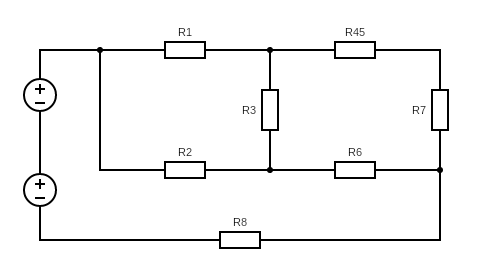
\includegraphics[scale=0.6,keepaspectratio]{fig/c1.png} \\
\end{center}

\noindent Rezistory $R_4$ a  $R_5$ zjednodušíme do jedného rezistora $R_{45}$ pomocou vzorca pre paralelne zapojené rezistory. \\

\begin{gather*}
	R_{45} = \frac{R_4 \times R_5}{R_4 + R_5} = \frac{440 \times 450}{440 + 450} = 222,4719 \Omega
\end{gather*}

\newpage

\begin{center}
\textbf{Krok 2} - Využitie metódy \textbf{Trojuholník - Hviezda}
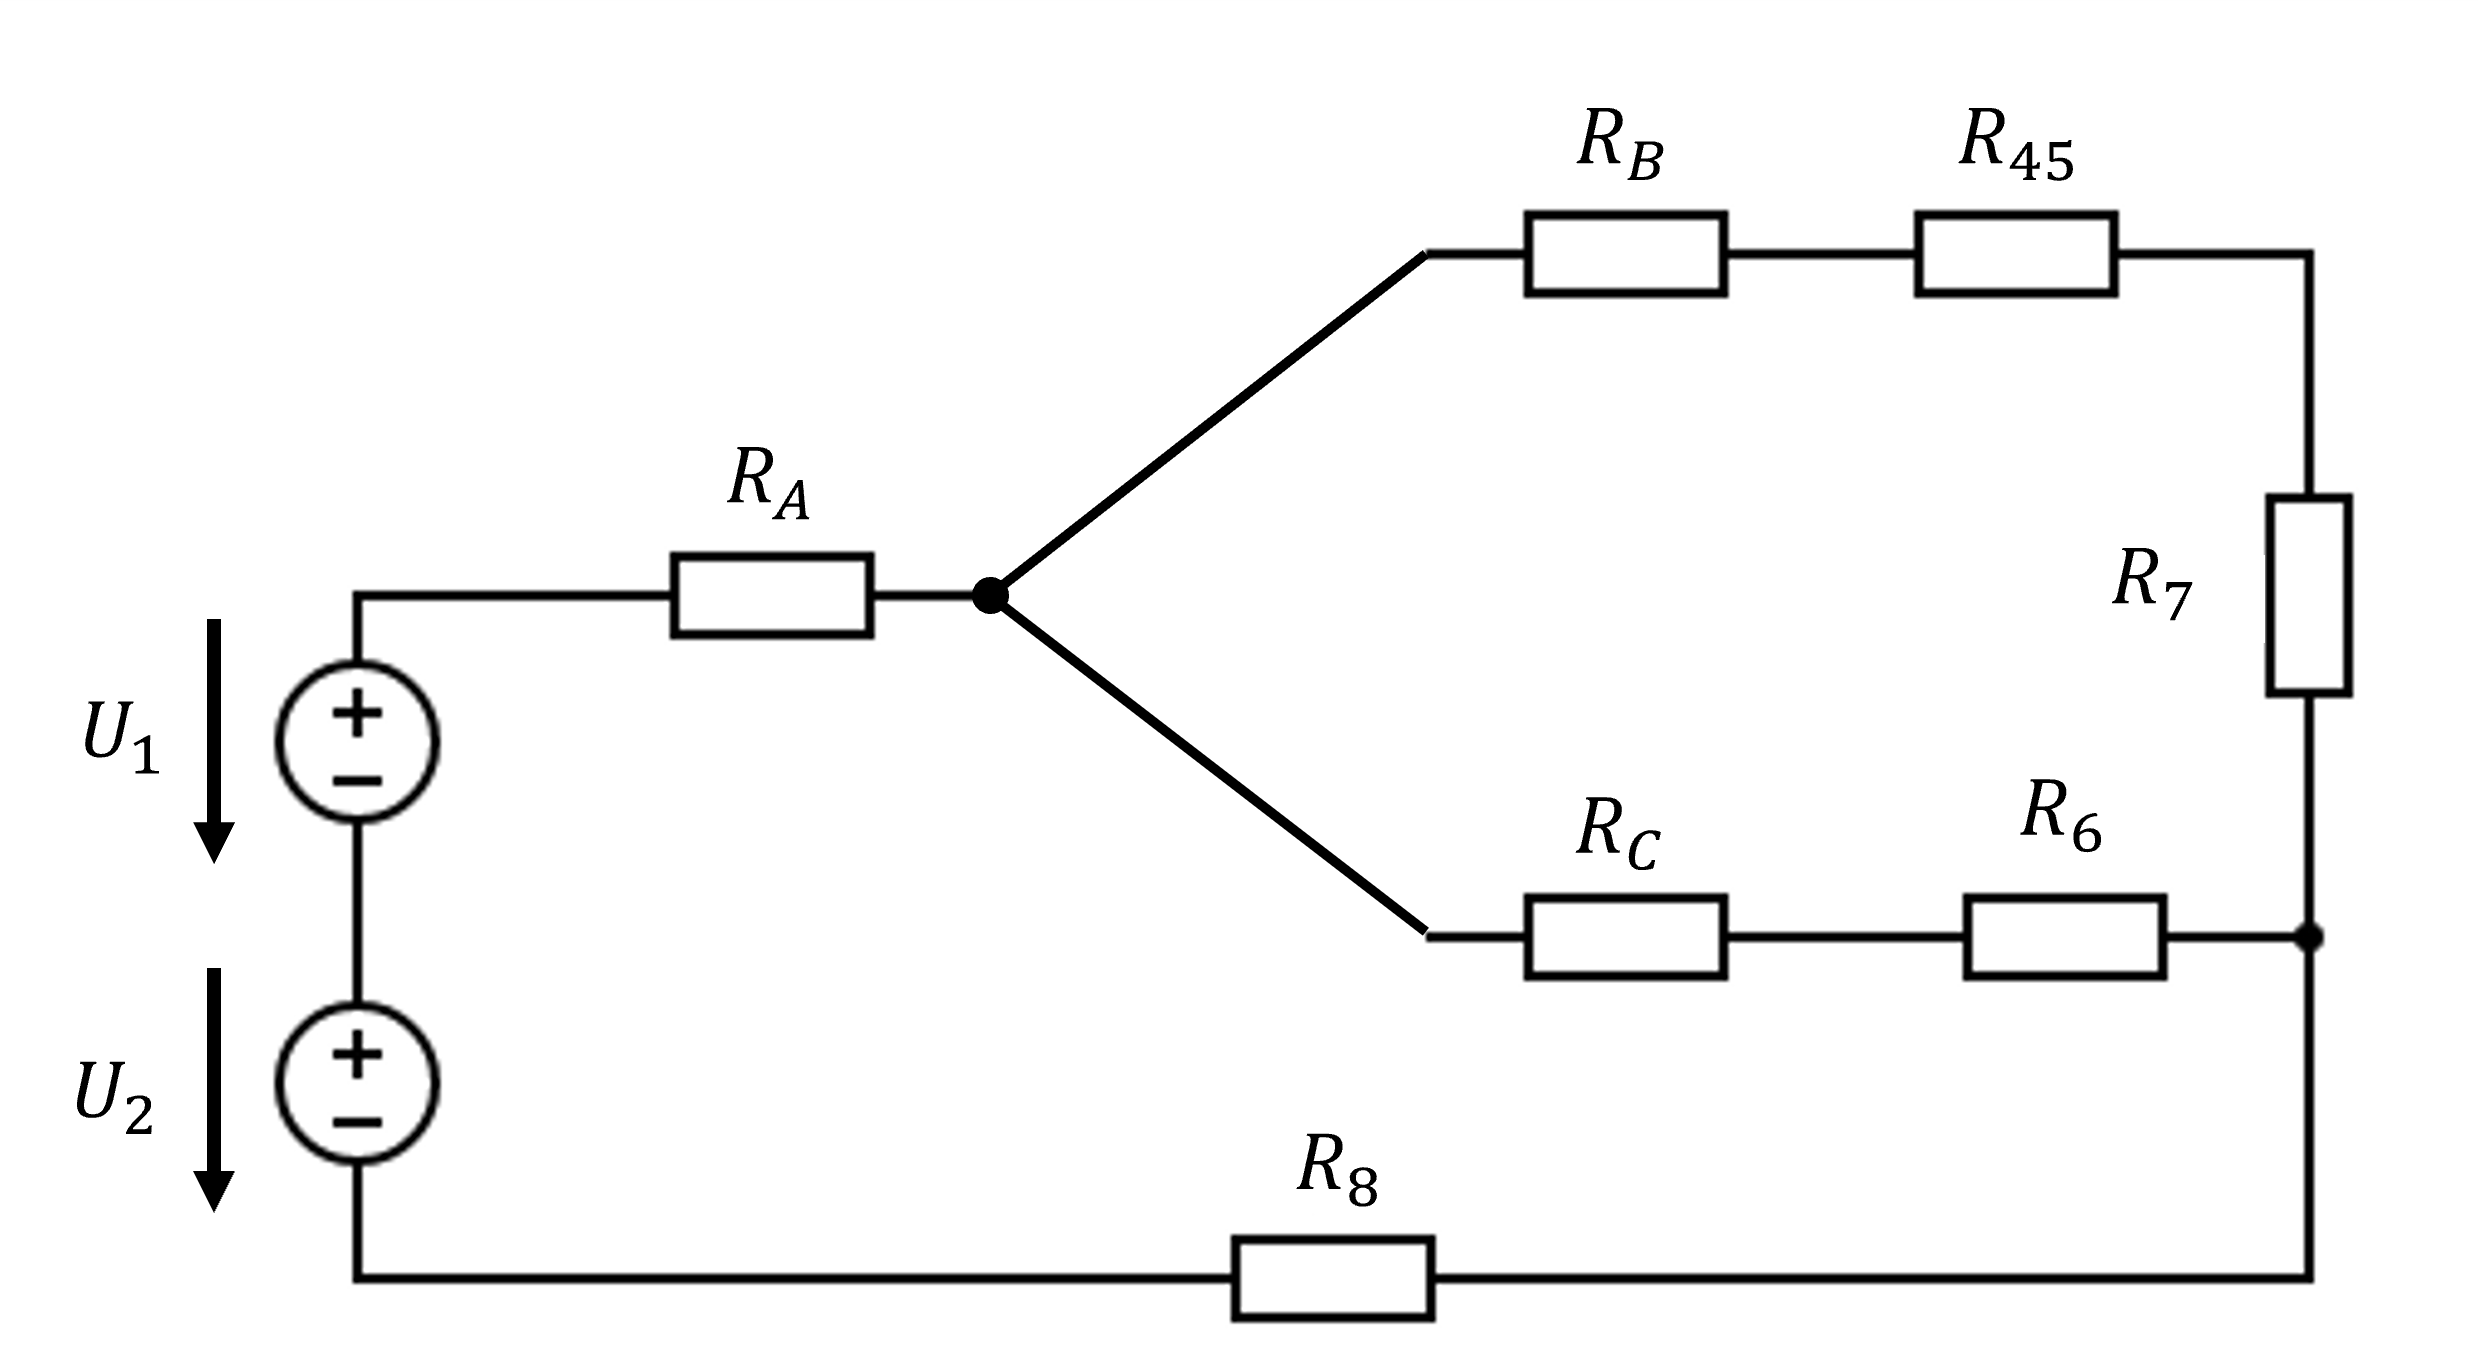
\includegraphics[scale=0.6,keepaspectratio]{fig/c2.png} \\
\end{center}

\noindent Z rezistorov $R_1$, $R_2$ a $R_3$ prevedieme z trojuholníka do hviezdy vypočítame hodnoty $R_A$, $R_B$ a $R_C$.\\

\begin{gather*}
R_A = \frac{R_1 \times R_2}{R_1 + R_2 + R_3} =
\frac{380 \times 420}{380 + 420 + 330}=
141.2389 \Omega \\\\
R_B = \frac{R_1 \times R_3}{R_1 + R_2 + R_3} =
\frac{380 \times 330}{380 + 420 + 330} =
110,9735 \Omega \\\\
R_C = \frac{R_2 \times R_3}{R_1 + R_2 + R_3} =
\frac{420 \times 330}{380 + 420 + 330} =
122,6549 \Omega \\\
\end{gather*}

\begin{center}
\textbf{Krok 3} -Sčítanie rezistorov $R_B$, $R_{45}$ a $R_7$ zapojených v sérii
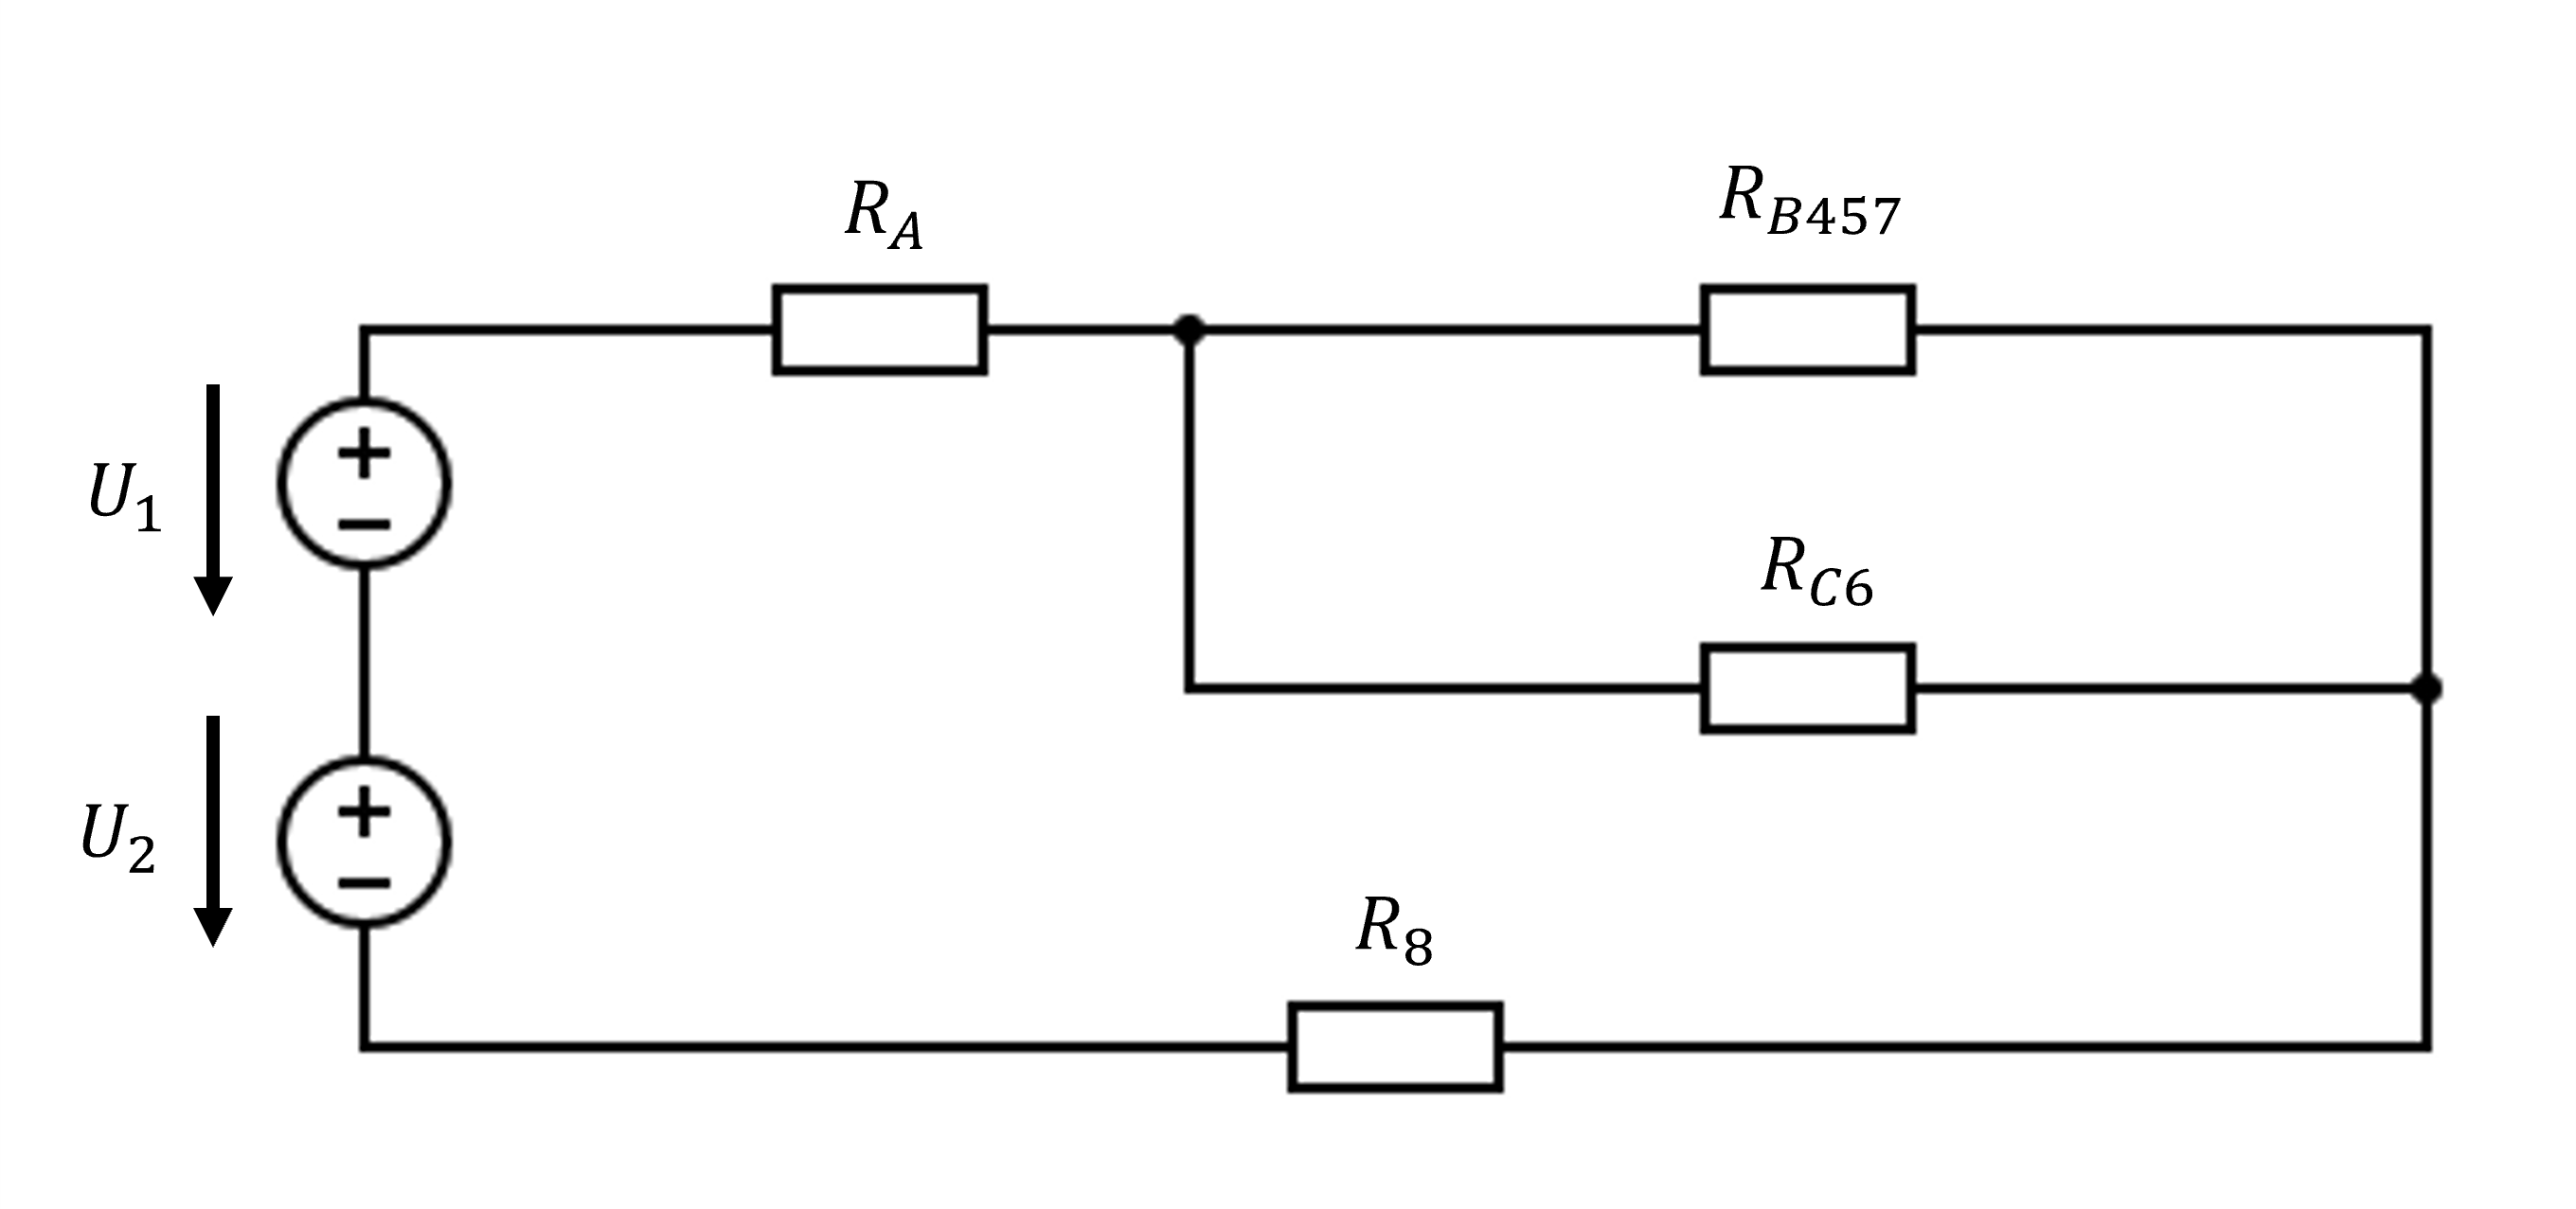
\includegraphics[scale=0.5,keepaspectratio]{fig/c3.png} \\
\end{center}

\begin{gather*}
R_{B457} = R_B + R_45 + R_7 =
110,9735 + 222.4719 + 410 =
743,4454 \Omega
\\\\
R_{C6} = R_C + R_6 =
122,6549 + 650 =
772.6549 \Omega
\\\
\end{gather*}
 
\newpage

\begin{center}
\textbf{Krok 4} - Zjednodušenie paralelne zapojených rezistorov $R_{B457}$ a $R_{C6}$ \\
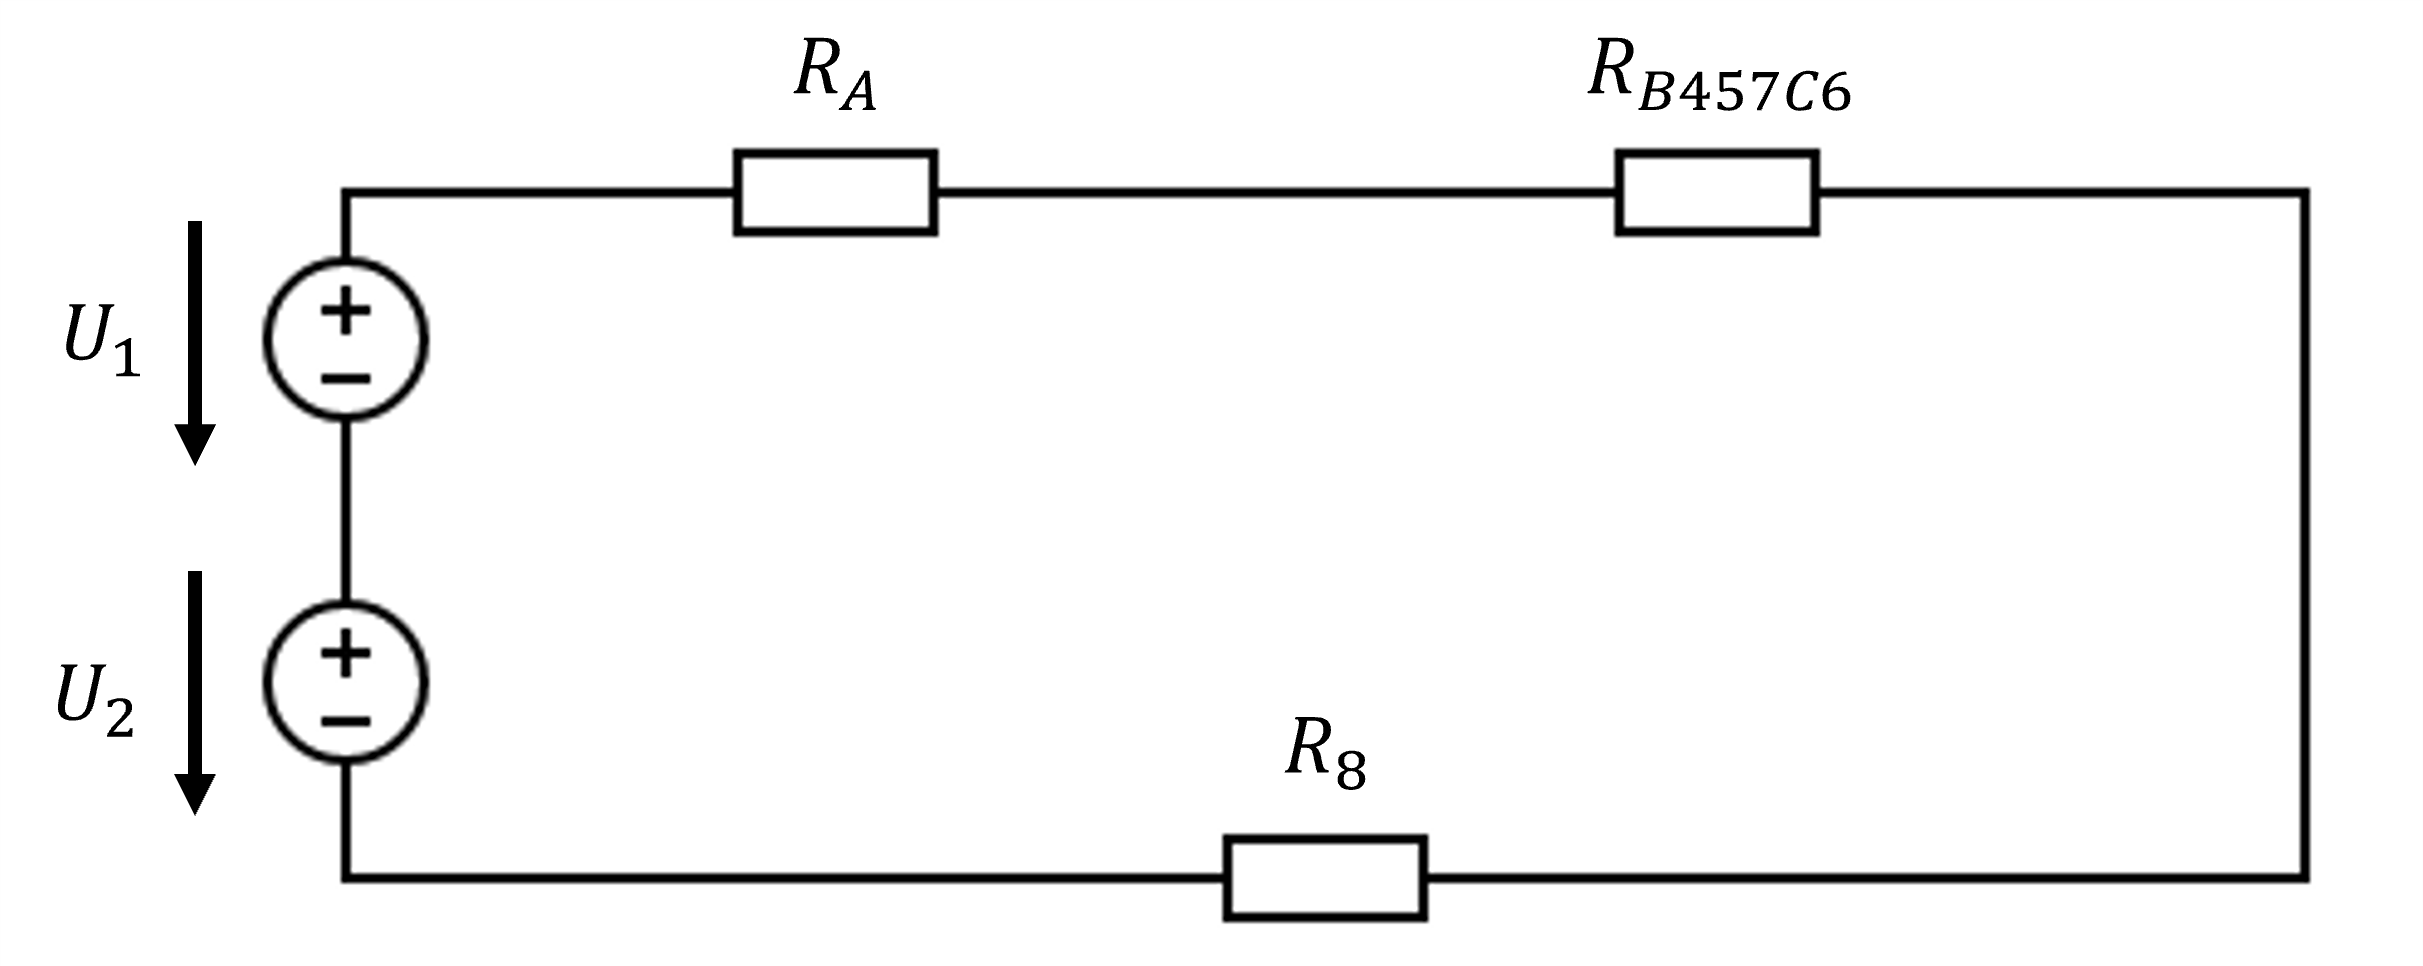
\includegraphics[scale=0.5,keepaspectratio]{fig/c4.png} \\
\end{center}

\begin{gather*}
    R_{B457C6} = \frac{R_{B457} \times R_{C6}}{R_{B457} + R_{C6}} =
    \frac{743,4454 \times 772.6549}{743,4454 +772.6549} =
    378,8844 \Omega \\
\end{gather*}

\begin{center}
\textbf{Krok 5} - Sčítanie sériových zdrojov $U_1$ a $U_2$
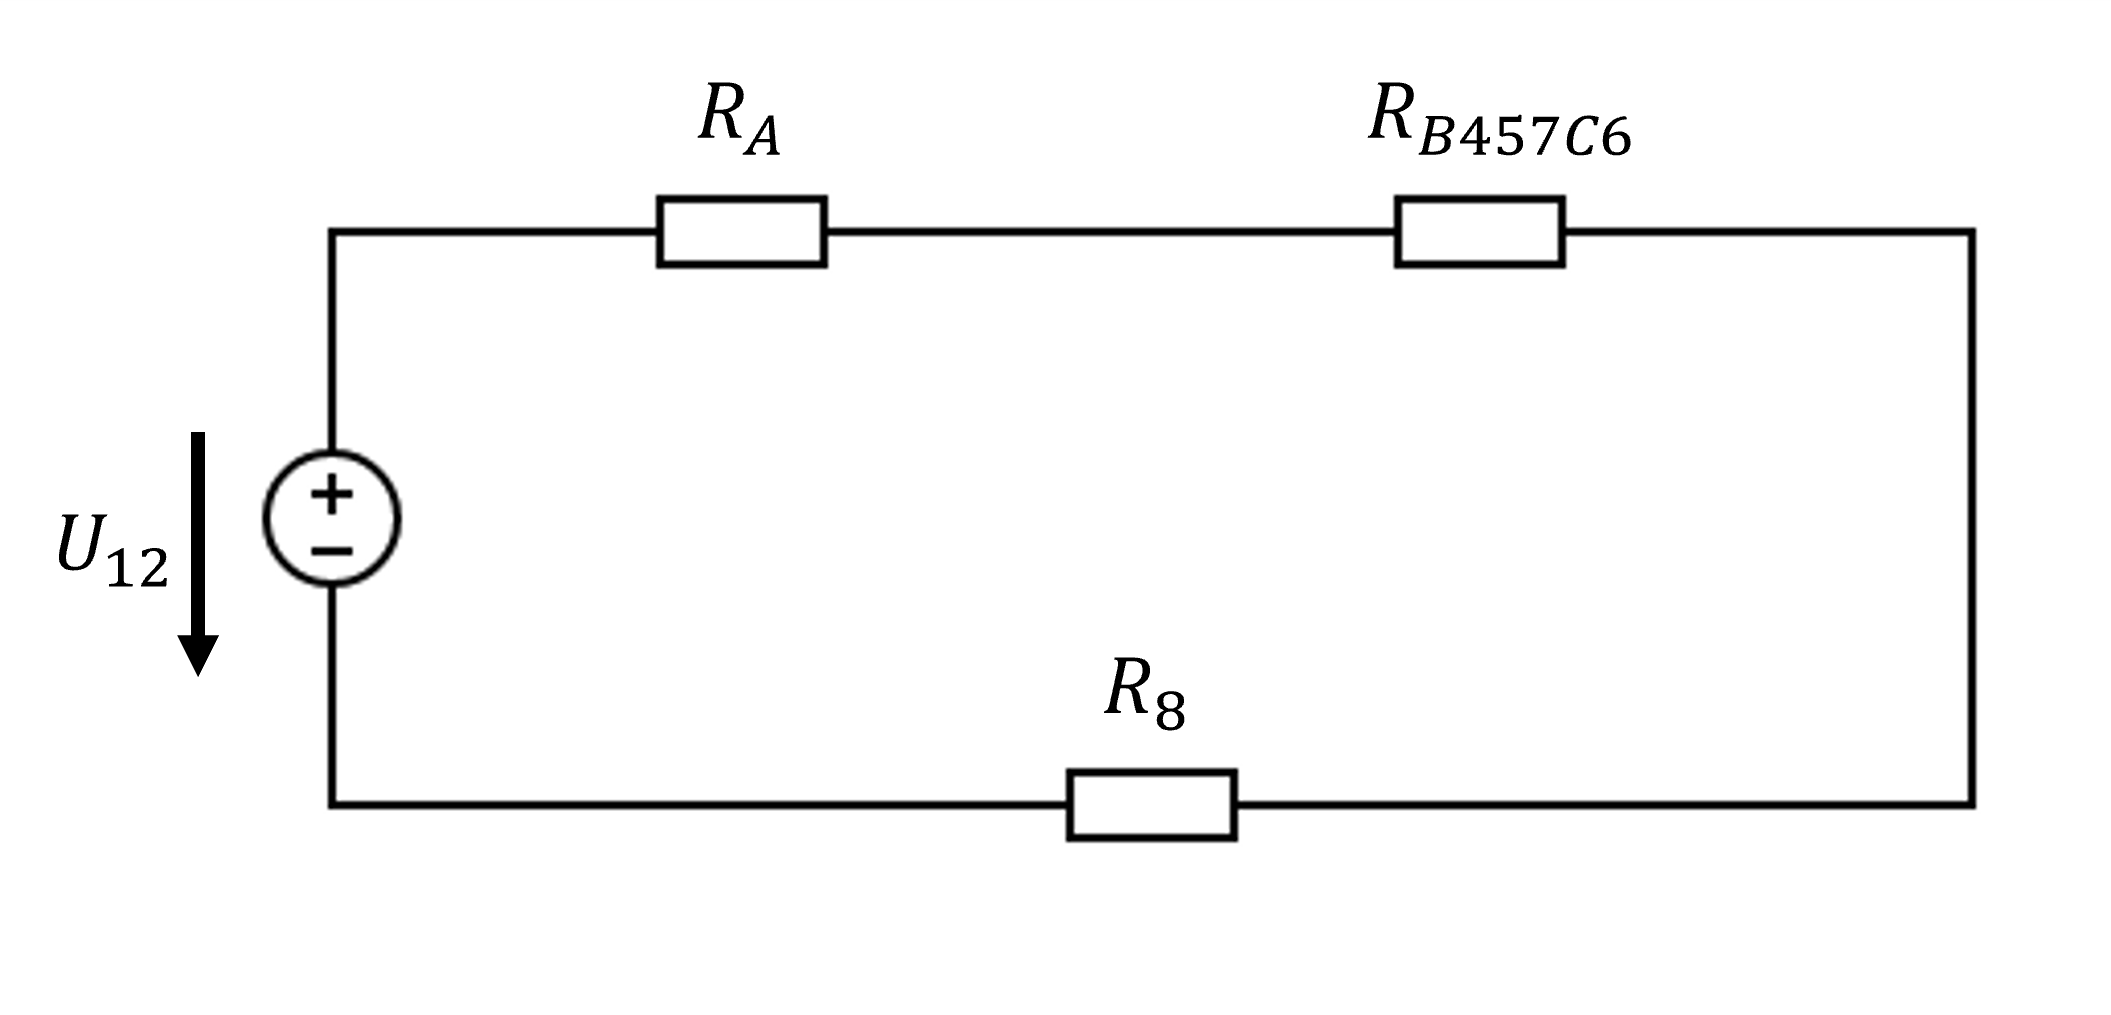
\includegraphics[scale=0.7,keepaspectratio]{fig/c5.png} \\
\end{center}

\begin{gather*}
   U_{12} = U_{1} + U_{2} = 130 + 60 = 190 V \\
\end{gather*}

\begin{center}
\textbf{Krok 6} - Výpočet R$_E$$_K$$_V$ - sčítanie sériových rezistorov $R_{B457C6}$, $R_A$ a $R_8$
\\
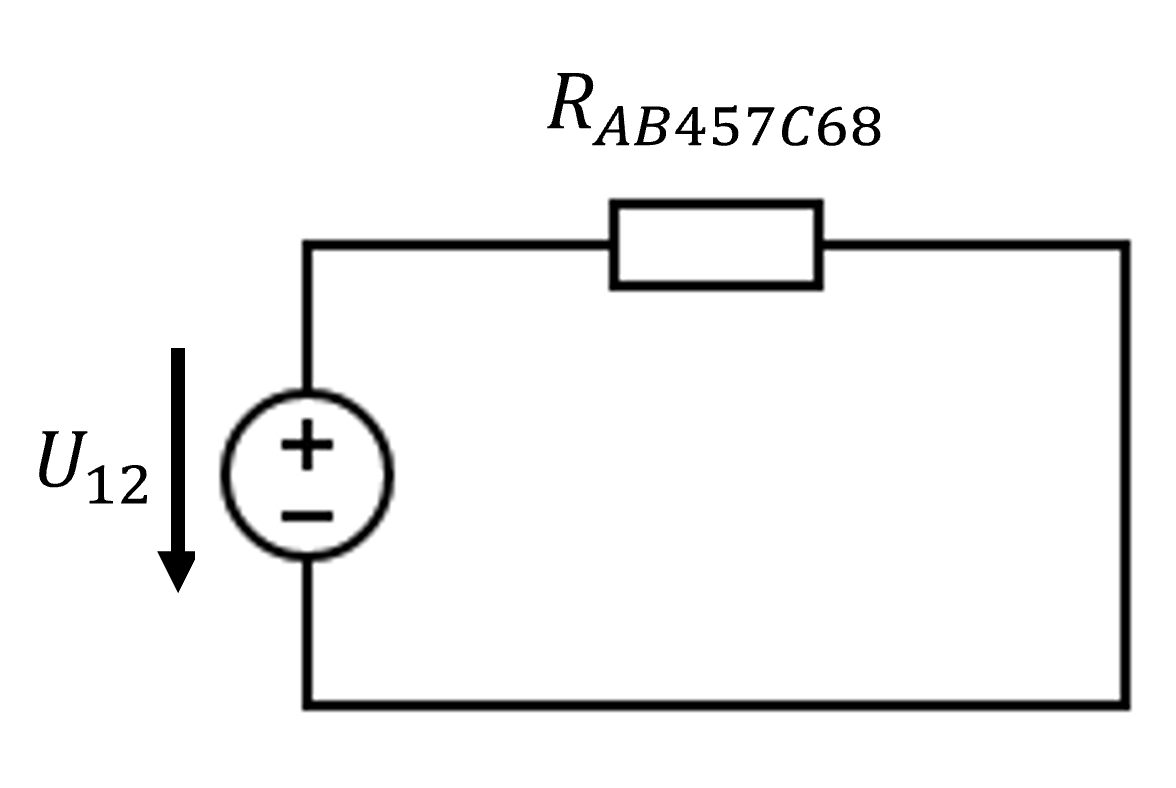
\includegraphics[scale=0.8,keepaspectratio]{fig/c6.png} \\
\end{center}

\noindent Ostávajúce sériové rezistory zjednodušíme do jedného rezistora označeného ako $R_{EKV}$ 

\begin{gather*}
    R_{EKV} = R_{A} + R_{B457C6} + R_{8} = 141,2389 + 378.8844 + 275 = 795,1233 \Omega
\end{gather*}

\newpage

\begin{center}
\textbf{Krok 7} - Výpočet prúdu pomocou Ohmovho zákona a $R_{EKV}$
\end{center}

\begin{gather*}
   I = \frac {U_{12}} {R_{EKV}} = \frac {190} {795,1233} = 0.23895 A \\
\end{gather*}

\begin{center}
\textbf{Krok 8} - Výpočet $U_{R_{7}}$ a $I_{R_{7}}$
\end{center}

Vypočítame si napätie na $R_{B457C6}$ pomocou prúdu $\boldsymbol{I}$, ktorý je v sériovom zapojení rovnaký na každom rezistore v danom obvode.

\begin{gather*}
    U_{R_{B457C6}} = I \times R_{B457C6} = 0.23895 \times 378,8844 = 90,5344 V \\
\end{gather*}

\noindent Ďalej vieme, že napätie prechádzajúce cez paralelné rezistory je na týchto rezistoroch taktiež rovnaké a pomocou toho dopočítame prúd na $\boldsymbol{R_{B457}}$

\begin{gather*}
    \boldsymbol{U_{R_{B457}}} = U_{R_{B457C6}} = 90,5334 V \\
\end{gather*}

\noindent Pomocou Omhovho zákona vieme dopočítať prúd na $\boldsymbol{R_{B457}}$

\begin{gather*}
   \boldsymbol{I_{R_{B457}}} = \frac {U_{R_{B457}}} {R_{B457}} = \frac{90,5334} {743,4454} = 0,12177 A \\
\end{gather*}

\noindent Pomocou $\boldsymbol{I_{R_{B457}}}$ a Ohmovho zákona už vieme dopočítať $\boldsymbol{U_{R_{7}}}$ a $\boldsymbol{I_{R_{7}}}$

\begin{gather*}
   \boldsymbol{I_{R_{7}}} = I_{R_{B457}} = \boldsymbol{0,12177 A} \\
   \boldsymbol{U_{R_{7}}} = I_{R_{7}} \times {R_{7}} = 0,12177 \times 410 = \boldsymbol{49,9279 V} \\
\end{gather*}

 

